   
\documentclass[11pt]{article}
\renewcommand{\baselinestretch}{1.05}
\usepackage{amsmath,amsthm,verbatim,amssymb,amsfonts,amscd, graphicx}
\usepackage{graphics}
\usepackage{mathtools}
\usepackage{listings}
\topmargin0.0cm
\headheight0.0cm
\headsep0.0cm
\oddsidemargin0.0cm
\textheight23.0cm
\textwidth16.5cm
\footskip1.0cm
\theoremstyle{plain}
\newtheorem{theorem}{Theorem}
\newtheorem{corollary}{Corollary}
\newtheorem{lemma}{Lemma}
\newtheorem{proposition}{Proposition}
\newtheorem*{surfacecor}{Corollary 1}
\newtheorem{conjecture}{Conjecture} 
\newtheorem{question}{Question} 
\theoremstyle{definition}
\newtheorem{definition}{Definition}
\DeclareMathOperator*{\argmax}{argmax}
 \begin{document}
 
\title{Report Artificial Intelligence, Project Section 2.B}
\date{}
\author{Domenico Alfano}
\maketitle

The report describes the results obtained during the development of Project Section 2.B. The main goal of this project has been to evaluate the capabilities and functionalities of some Reinforcement Learning Algorithms applied in BlackJack Problem.

\section{Introduction}
Blackjack is a popular card game played in many casinos. The objective of the game is to win money by obtaining a point total higher than the dealer's without exceeding 21. Determining an optimal blackjack strategy proves to be a difficult challenge due to the stochastic nature of the game. This presents an interesting opportunity for machine learning algorithms. Supervised learning techniques may provide a viable solution, but do not take advantage of the inherent reward structure of the game. Reinforcement learning algorithms generally perform well in stochastic environments. I have modified the problem to simplify the original BlackJack card game; the changes of the rules and the assumptions maded are described in the Domain Description of the problem.

\section{Description of the problem}
As I said before, the rules of the card game are different according to my changes and are shown below:
\begin{itemize}
\item The game is played with an infinite deck of cards.
\item Each draw from the deck results in a value between 1 and 10 (uniformly distributed) with a colour of red (probability 1/3) or black (probability 2/3).
\item There are no aces or picture (face) cards in this game (For the management of the aces cards I assume that they can take only the value 1).
\item At the start of the game both the player and the dealer draw one black card (fully observed).
\item Each turn the player may either stick or hit.
\item If the player hits then she draws another card from the deck, if the player sticks she receives no further cards.
\item The values of the player’s cards are added (black cards) or subtracted (red cards).
\item If the player’s sum exceeds 21, or becomes less than 1, then she “goes bust” and loses the game (reward -1).
\item If the player sticks then the dealer starts taking turns. The dealer always sticks on any sum of 17 or greater, and hits otherwise. If the dealer goes bust, then the player wins; otherwise, the outcome – win (reward +1), lose (reward -1), or draw (reward 0) – is the player with the largest sum.
\end{itemize}

\section{Formal model of the problem}
We play a simplest version of Blackjack with an infinite deck of cards. (The infinite deck assumption ensures that the probability of drawing any specific card is equal all times, independent of our hand, but depending.) The game of Blackjack proceeds in rounds. We can decide in each round whether to be dealt another card (hit) or stick with our current hand and bet (stick), which ends the game. We win if the sum of face values of cards in our hand is below 21 and closer to 21 than the hand of the bank player (who usually plays according to some fixed and publicly known rules, i.e., takes another card until the sum of face values exceeds some predefined threshold,, in our case 17).
We can formulate this game as a MDP $<S,A,T,R>$ (There is no discounting, $\gamma = 1)$in the following way:

\begin{itemize}
\item \textbf{States}: (P,D) where
\begin{itemize}
\item P: current sum of player card values.
\item D: current sum of dealer (when is at least 17, the dealer stop to HIT)
\end{itemize}
\item \textbf{Action}: {HIT, STICK} (the player HIT when he wants another card, stay if he is satisfied of the value of the sum)
\item \textbf{Transition function}:
\begin{table}[h]
\centering
\caption{Transition table}
\label{my-label}
\begin{tabular}{lll}
State & Action & Transition    \\
(P,D) & STICK   & (P,D)         \\
(P,D) & HIT    & (P $\cup$ ${c}$, D)
\end{tabular}
\end{table}
where c is the value of new card extracted.
\item \textbf{Reward}:  If the dealer goes bust, then the player wins; otherwise, the outcome – win (reward +1), lose (reward -1), or draw (reward 0) – is the player with the largest sum.

 
\end{itemize}

%I have formalized the problem as follow:
%The state of the model is the state of the game: It represent the current sum of the player and the first card of the dealer;
%–  current sum (12-21) 
%–  dealer’s showing card (ace, 2-10) 
%The set of action is:
%$A={HIT, STIK}$
%The transition function is formalized as follow:
%$X \times A \rightarrow X' \in X$ 
\newpage
\section{Solution algorithms}

The Solution Algorithms chosen are: Monte Carlo method and a Temporal Difference($\lambda$) Algorithm's such as Sarsa($\lambda$).

\subsection{Monte Carlo Control}
In this section we consider our first learning methods for estimating value functions and discovering optimal policies. Here we do not assume complete knowledge of the environment. Monte Carlo methods require only experience-sample sequences of states, actions, and rewards from on-line or simulated interaction with an environment. Learning from on-line experience is striking because it requires no prior knowledge of the environment's dynamics, yet can still attain optimal behavior. Learning from simulated experience is also powerful. Although a model is required, the model need only generate sample transitions, not the complete probability distributions of all possible transitions that is required by dynamic programming (DP) methods. In surprisingly many cases it is easy to generate experience sampled according to the desired probability distributions, but infeasible to obtain the distributions in explicit form.
\\
Monte Carlo methods are ways of solving the reinforcement learning problem based on averaging sample returns. To ensure that well-defined returns are available, we define Monte Carlo methods only for episodic tasks. That is, we assume experience is divided into episodes, and that all episodes eventually terminate no matter what actions are selected. It is only upon the completion of an episode that value estimates and policies are changed. 
\\
Monte Carlo methods are thus incremental in an episode-by-episode sense, but not in a step-by-step sense. The term "Monte Carlo" is often used more broadly for any estimation method whose operation involves a significant random component. Here we use it specifically for methods based on averaging complete returns
\\
We begin by considering Monte Carlo methods for learning the state-value function for a given policy. Recall that the value of a state is the expected return--expected cumulative future discounted reward--starting from that state. An obvious way to estimate it from experience, then, is simply to average the returns observed after visits to that state. As more returns are observed, the average should converge to the expected value. This idea underlies all Monte Carlo methods.
\\
In particular, suppose we wish to estimate $V^\pi(s)$, the value of a state $s$ under policy $\pi$, given a set of episodes obtained by following $\pi$  and passing through $s$.
\\
Therefore the following equation show the updating of Value Function:
\begin{equation}
V(s_t) \leftarrow V(s_t) + \alpha [R_t -  V(s_t)]
\end{equation}
where $R_t$ is the actual long-term return following state $s_t$, as we can see in the following Figure.
\begin{center}
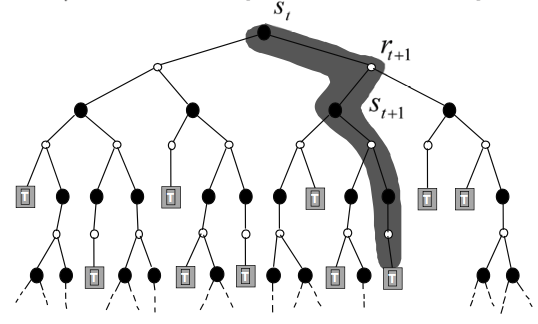
\includegraphics[scale=0.7]{1}
\end{center}
We are now ready to consider how Monte Carlo estimation can be used in control, that is, to approximate optimal policies. The overall idea is to proceed according to the idea of generalized policy iteration (GPI). In GPI one maintains both an approximate policy and an approximate value function. The value function is repeatedly altered to more closely approximate the value function for the current policy, and the policy is repeatedly improved with respect to the current value function as in the following Figure:
\begin{center}
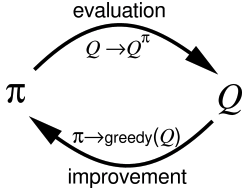
\includegraphics[scale=0.7]{2}
\end{center}
These two kinds of changes work against each other to some extent, as each creates a moving target for the other, but together they cause both policy and value function to approach optimality.
\\
To better understand how Monte Carlo works, we can consider a simple example:
\\
Consider a Monte Carlo version of classical policy iteration. In this method, we perform alternating complete steps of policy evaluation and policy improvement, beginning with an arbitrary policy $\pi_0$ and ending with the optimal policy and optimal action-value function:
\begin{equation}
\pi_0\xrightarrow{\text{E}}Q^{\pi_0}\xrightarrow{\text{I}}\pi_1\xrightarrow{\text{E}}Q^{\pi_1}\xrightarrow{\text{I}}\pi_2\xrightarrow{\text{E}}\cdots\xrightarrow{\text{I}}\pi^*\xrightarrow{\text{E}}Q^{*},
\end{equation}
where $\xrightarrow{\text{E}}$ denotes a complete policy evaluation and $\xrightarrow{\text{I}}$ denotes a complete policy improvement.
\newpage
Under these assumptions, the Monte Carlo methods will compute each $Q^{\pi_k}$ exactly, for arbitrary ${\pi_k}$.
Policy improvement is done by making the policy greedy with respect to the current value function. In this case we have an action-value function, and therefore no model is needed to construct the greedy policy. For any action-value function $Q$, the corresponding greedy policy is the one that, for each $s \in S$ , deterministically chooses an action with maximal $Q$-value: 
\begin{equation}
\pi(s)=\argmax_a Q(s,a)
\end{equation}
Policy improvement then can be done by constructing each $\pi_{k+1}$ as the greedy policy with respect to $Q^{\pi_k}$ . The policy improvement theorem then applies  to $\pi_k$  and $\pi_{k+1}$ because, for all $s \in S$ , 

\begin{equation}
\begin{split}
Q^{\pi_k}(s, \pi_{k+1}(s))=Q^{\pi_k}(s, \argmax_a Q^{\pi_k}(s,a)) \\
= \max_a Q^{\pi_k}(s,a) \hspace{1.8cm} \\
\geq Q^{\pi_k}(s,\pi_k (s)) \hspace{1.9cm} \\
= V^{\pi_k} (s) \hspace{2.8cm}
\end{split}
\end{equation}
The theorem assures us that each $\pi_{k+1}$ is uniformly better than $\pi_k$ , unless it is equal to $\pi_k$ , in which case they are both optimal policies.

\subsection{Temporal Difference Learning}
Temporal Difference (TD) Learning is a combination of Monte Carlo ideas and dynamic programming (DP) ideas. Like Monte Carlo methods, TD methods can learn directly from raw experience without a model of the environment's dynamics. Like DP, TD methods update estimates based in part on other learned estimates, without waiting for a final outcome. The relationship between TD and Monte Carlo methods is a recurring theme in the theory of reinforcement learning.
\\
As usual, we start by focusing on the policy evaluation or prediction problem, that of estimating the value function  $V^\pi(s)$ for a given policy $\pi$. For the control problem (finding an optimal policy), TD and Monte Carlo methods all use some variation of generalized policy iteration (GPI). The differences in the methods are primarily differences in their approaches to the prediction problem.
\\
Whereas Monte Carlo methods must wait until the end of the episode to determine the increment to $V(s_t)$ (only then is $R_t$ known), TD methods need wait only until the next time step. At time $t+1$ they immediately form a target and make a useful update using the observed reward $r_{t+1}$ and the estimate $V(s_{t+1})$. \\
The simplest TD method, known as $TD(0)$, is:
\begin{equation}
V(s_t) \leftarrow V(s_t) + \alpha [r_{t+1}+\gamma V(s_{t+1})-V(s_t)]
\end{equation}
In effect, the target for the Monte Carlo update is $R_t$, whereas the target for the TD update is $r_{t+1}+\gamma V(s_{t+1})$ .
\newpage
\subsubsection{SARSA}
We turn now to the use of TD prediction methods for the control problem. As usual, we follow the pattern of generalized policy iteration (GPI), only this time using TD methods for the evaluation or prediction part. As with Monte Carlo methods, we face the need to trade off exploration and exploitation, and again approaches fall into two main classes: $on-policy$ and $off-policy$. In this section we present an on-policy TD control method, Sarsa.
The first step is to learn an action-value function rather than a state-value function. In particular, for an on-policy method we must estimate $Q^\pi (s,a)$  for the current behavior policy $\pi$  and for all states $s$  and actions $a$ . This can be done using essentially the same TD method described above for learning $V^\pi$.\\

In the previous section we considered transitions from state to state and learned the values of states. Now we consider transitions from state-action pair to state-action pair, and learn the value of state-action pairs. Formally these cases are identical: they are both Markov chains with a reward process. The theorems assuring the convergence of state values under $TD(0)$ also apply to the corresponding algorithm for action values: 
\begin{equation}
Q(s_t,a_t) \leftarrow Q(s_t,a_t) + \alpha [r_{t+1}+\gamma Q(s_{t+1},a_{t+1})-Q(s_t,a_t)]
\end{equation}
This update is done after every transition from a nonterminal state $s_t$. If $s_{t+1}$ is terminal, then $Q(s_{t+1},a_{t+1})$ is defined as zero.\\

This rule uses every element of the quintuple of events, $(s_t ,a_t ,r_{t+1} ,s_{t+1},a_{t+1})$, that make up a transition from one state-action pair to the next. \\

This quintuple gives rise to the name Sarsa for the algorithm.\\

It is straightforward to design an on-policy control algorithm based on the Sarsa prediction method. As in all on-policy methods, we continually estimate $Q^\pi$ for the behavior policy $\pi$, and at the same time change $\pi$ toward greediness with respect to  $Q^\pi$. 
\subsubsection{Eligibility Trace}
Eligibility Trace are one of the basic mechanisms of reinforcement learning. For example, in the popular TD($\lambda $) algorithm, the $\lambda $ refers to the use of an eligibility trace. Almost any temporal-difference (TD) method, such as Q-learning or Sarsa, can be combined with eligibility traces to obtain a more general method that may learn more efficiently.
The Eligibility Trace could be viewed as a bridge from TD to Monte Carlo methods. When TD methods are augmented with eligibility traces, they produce a family of methods spanning a spectrum that has Monte Carlo methods at one end and one-step TD methods at the other. In between are intermediate methods that are often better than either extreme method. In this sense eligibility traces unify TD and Monte Carlo methods in a valuable and revealing way.

There are two different types of Eligibility Trace: 
\begin{itemize}
\item Forward view of TD($\lambda$): For each state visited, we look forward in time to all the future rewards and decide how best to combine them. We might imagine ourselves riding the stream of states, looking forward from each state to determine its update, as suggested by the following Figure. After looking forward from and updating one state, we move on to the next and never have to work with the preceding state again. Future states, on the other hand, are viewed and processed repeatedly, once from each vantage point preceding them.

\begin{center}
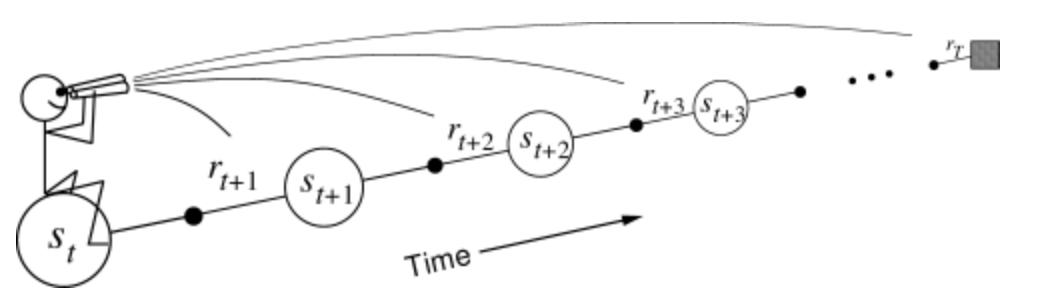
\includegraphics[scale=0.7]{3}
\end{center}

\item Backward view of TD($\lambda $): is oriented backward in time. At each moment we look at the current TD error and assign it backward to each prior state according to the state's eligibility trace at that time. We might imagine ourselves riding along the stream of states, computing TD errors, and shouting them back to the previously visited states, as suggested by the following Figure.

\begin{center}
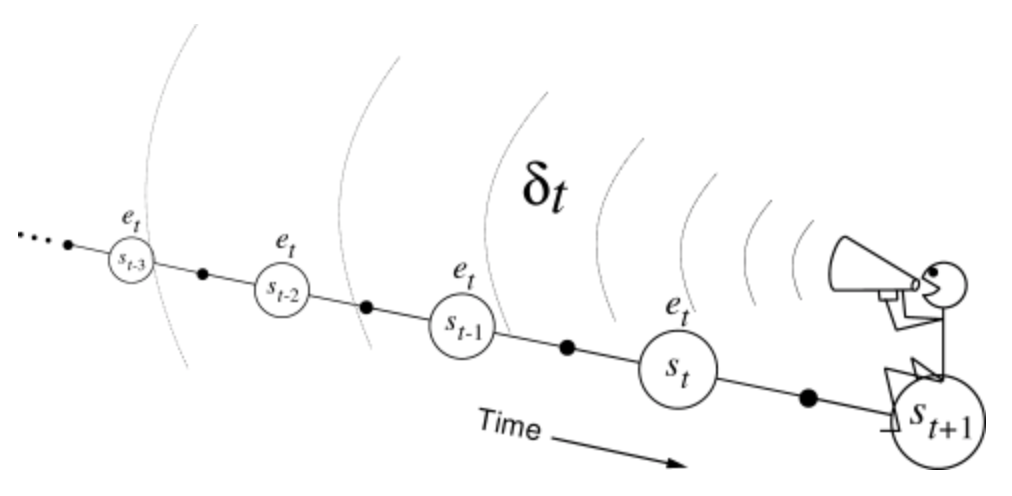
\includegraphics[scale=0.7]{4}
\end{center}

\end{itemize}

In the backward view of TD($\lambda $), there is an additional memory variable associated with each state, its Eligibility Trace. The eligibility trace for state $s$ at time $t$  is denoted $e_t(s) \in \mathbb{R}^+$ . On each step, the eligibility traces for all states decay by $\gamma^\lambda$ , and the eligibility trace for the one state visited on the step is incremented by 1:

\begin{equation}
e_t(s) = 
\begin{cases}
\gamma^\lambda e_{t-1}(s) \hspace{3cm} if \hspace{0.2cm} s \neq s_t;\\
\gamma^\lambda e_{t-1}(s)+1 \hspace{2.3cm} if  \hspace{0.2cm}  s = s_t;
\end{cases}
\end{equation} 

for all nonterminal states $s$ , where $\lambda$  is the discount rate and  is the parameter introduced in the previous section. Henceforth we refer to $\lambda $ as the trace-decay parameter. This kind of eligibility trace is called an accumulating trace because it accumulates each time the state is visited, then fades away gradually when the state is not visited.\\
At any time, the traces record which states have recently been visited, where "recently" is defined in terms of . The traces are said to indicate the degree to which each state is eligible for undergoing learning changes should a reinforcing event occur. The reinforcing events we are concerned with are the moment-by-moment one-step TD errors. For example, the TD error for state-value prediction is:
\begin{equation}
\delta_t= r_{t+1} + \gamma V_t(s_{t+1}) - V_t(s_t)
\end{equation} 
To better understand the backward view, consider what happens at various values of $\lambda $. If $\lambda=0 $ , then by (8) all traces are zero at $t$ except for the trace corresponding to $s_t$. For larger values of $\lambda $, but still $\lambda <1$, more of the preceding states are changed, but each more temporally distant state is changed less because its eligibility trace is smaller.

If $\lambda=1$, then the credit given to earlier states falls only by $\gamma$ per step. This turns out to be just the right thing to do to achieve Monte Carlo behavior. For example, remember that the TD error, $\gamma_t$, includes an undiscounted term of $r_{t+1}$. In passing this back $k$ steps it needs to be discounted, like any reward in a return, by $\gamma^k$, which is just what the falling eligibility trace achieves. If $\lambda=1$ and $\gamma=1$, then the eligibility traces do not decay at all with time. In this case the method behaves like a Monte Carlo method for an undiscounted, episodic task. If $\lambda=1$, the algorithm is also known as TD(1).
\\
TD(1) is a way of implementing Monte Carlo algorithms that is more general than those presented earlier and that significantly increases their range of applicability. Whereas the earlier Monte Carlo methods were limited to episodic tasks, TD(1) can be applied to discounted continuing tasks as well. Moreover, TD(1) can be performed incrementally and on-line.\\
 One disadvantage of Monte Carlo methods is that they learn nothing from an episode until it is over. For example, if a Monte Carlo control method does something that produces a very poor reward but does not end the episode, then the agent's tendency to do that will be undiminished during the episode. On-line TD(1), on the other hand, learns in an -step TD way from the incomplete ongoing episode, where the  steps are all the way up to the current step. If something unusually good or bad happens during an episode, control methods based on TD(1) can learn immediately and alter their behavior on that same episode.

\subsubsection{SARSA($\lambda$)}
How can eligibility traces be used not just for prediction, as in TD($\lambda $), but for control? As usual, the main idea of one popular approach is simply to learn action values, $Q_t(s,a)$, rather than state values,$V_t(s)$ . In this section we show how eligibility traces can be combined with Sarsa in a straightforward way to produce an on-policy TD control method. The eligibility trace version of Sarsa we call Sarsa($\lambda $).

The idea in Sarsa($\lambda $) is to apply the TD($\lambda $) prediction method to state-action pairs rather than to states. Obviously, then, we need a trace not just for each state, but for each state-action pair. Let $e_t(s,a)$ denote the trace for state-action pair $(s,a)$ . Otherwise the method is just like TD($\lambda $), substituting state-action variables for state variables $Q(s,a)$ for $V(s)$  and $e_t(s,a)$ for $e_t(s)$ : 

\begin{equation}
Q_{t+1}(s,a) = Q_t(s,a)+\alpha \delta_t e_t(s,a) \hspace{1.5cm} for\hspace{0.1cm} all \hspace{0.1cm}s,a
\end{equation}

where

\begin{equation}
\delta_t = r_{t+1} + \gamma Q_t(s_{t+1},a_{t+1})-Q_t(s_t,a_t)
\end{equation}

and for all $s, a$

\begin{equation}
e_t(s) = 
\begin{cases}
\gamma^\lambda e_{t-1}(s,a)+1 \hspace{2.3cm} if  \hspace{0.2cm}  s = s_t \hspace{0.1cm}and \hspace{0.1cm}a=a_t;\\
\gamma^\lambda e_{t-1}(s,a) \hspace{3cm} \hspace{0.1cm} otherwise;
\end{cases}
\end{equation} 

\begin{center}
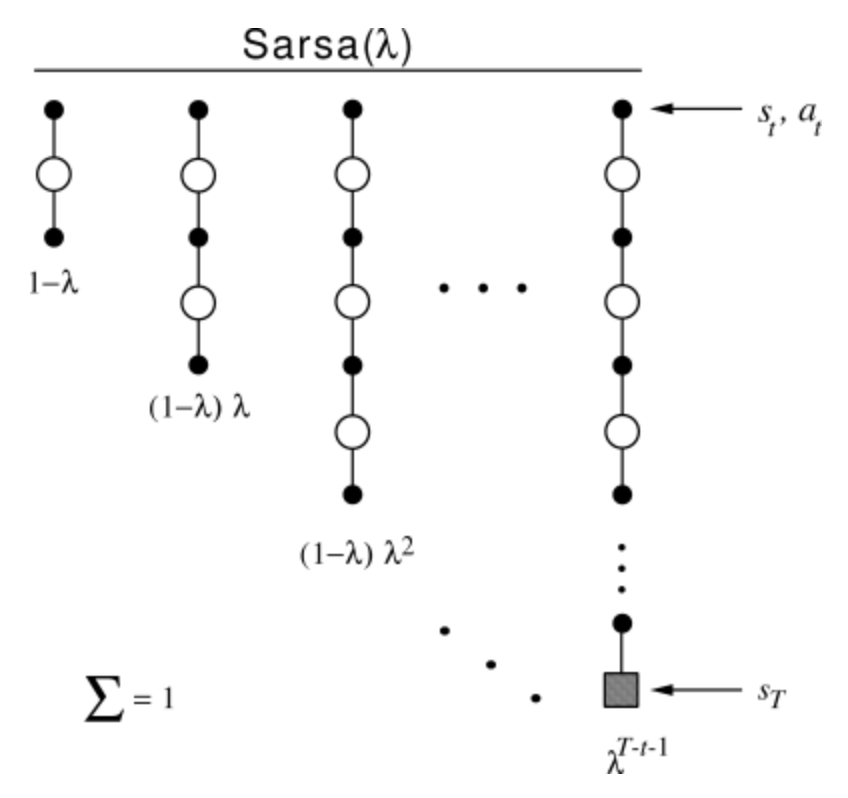
\includegraphics[scale=0.7]{6}
\end{center}

One-step Sarsa and Sarsa($\lambda $) are on-policy algorithms, meaning that they approximate $Q^\pi(s,a)$, the action values for the current policy,$\pi$ , then improve the policy gradually based on the approximate values for the current policy. The policy improvement can be done in many different ways; for example, the simplest approach is to use the $\varepsilon $-greedy policy with respect to the current action-value estimates. Next Figure shows the complete Sarsa($\lambda $) algorithm for this use case.

\begin{center}
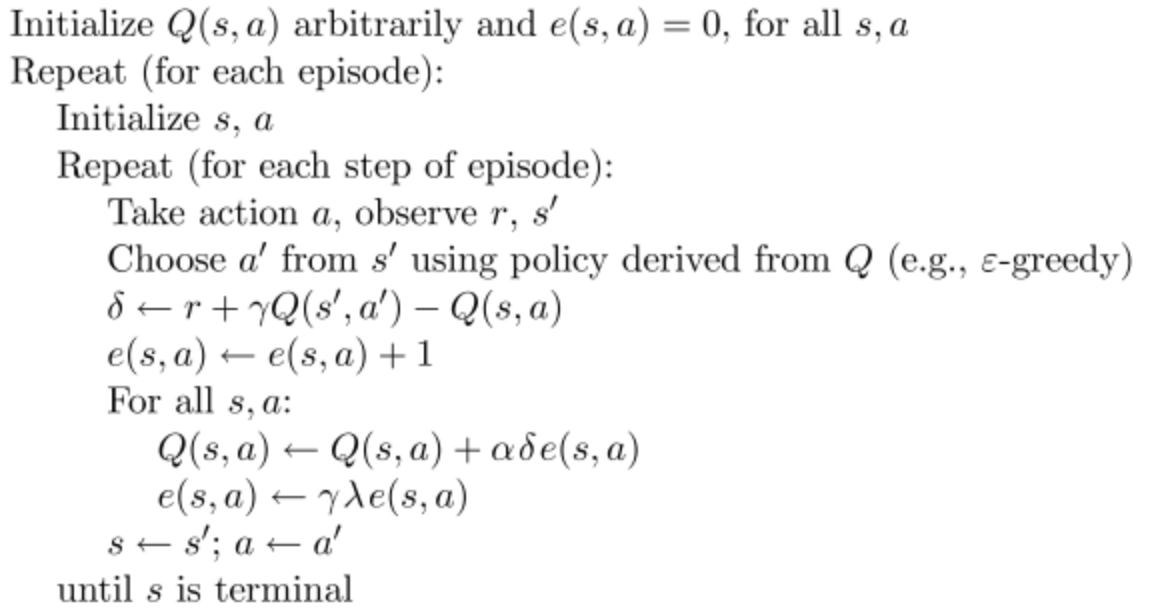
\includegraphics[scale=0.7]{5}
\end{center}

\section{Implementation}
The Monte Carlo implementation follow these steps:
\begin{itemize}
\item Initialise the value function to zero.
\item Use a time-varying scalar step-size of $\alpha_t  = 1/N (s_t , a_t )$
\item Use an $\varepsilon$-greedy exploration strategy with $\varepsilon_t = N_0 /(N_0 + N (s_t))$, where$ N_0 = 100$ is a constant, and $N(s,a)$ is the number of times that action a has been selected from state s.
\item No discounting ($\gamma$ = 1)
\end{itemize}

\begin{lstlisting}
def monte_carlo(iterations=100000, policy=policies.epsilon_greedy, n_zero=100):
   
    :param iterations: number of monte carlo iterations
    :param policy: exploration strategy to use
    :param n_zero: epsilon greedy constant
    (only applicable if epsilon greedy policy is used)
    :return: value function and the plot of the optimal value function
    
    Inizialization
    
    value_function = defaultdict(float)
   
    counter_state = defaultdict(int)
   
    counter_state_action = defaultdict(int)
    # number of wins
    wins = 0

    print('Iterations completed:')
    for i in xrange(iterations):

        if (i % 500000) == 0:
            print(i)

        # create a new random starting state
        state = environment.State()
        # play a round
        observed_keys = []
        while not state.terminal:
            player = state.player_sum
            dealer = state.dealer_first_card

            # find an action defined by the policy
            epsilon = n_zero / float(n_zero + counter_state[(player, dealer)])
            action = policy(epsilon, value_function, state)
            observed_keys.append((player, dealer, action))

            # take a step
            [state, reward] = environment.step(state, action)

        # we have reached an end of episode
        if reward is not None:
            # update over all keys
            for key in observed_keys:
                # update counts
                counter_state[key[:-1]] += 1
                counter_state_action[key] += 1

                # update value function
                alpha = 1.0 / counter_state_action[key]
                value_function[key] += alpha * (reward - value_function[key])

        if reward == 1:
            wins += 1

    print('Wins: %.4f%%' % ((float(wins) / iterations) * 100))
    # plot the optimal value function
    plotting.plot_value_function(value_function)
    return value_function

\end{lstlisting}

\newpage

The Sarsa$(\lambda)$ implementation follow these steps:
\begin{itemize}
\item Initialise the value function to zero.
\item Use a time-varying scalar step-size of $\alpha_t  = 1/N (s_t , a_t )$
\item Use an $\varepsilon$-greedy exploration strategy with $\varepsilon_t = N_0 /(N_0 + N (s_t))$, where$ N_0 = 100$ is a constant, and $N(s,a)$ is the number of times that action a has been selected from state s.
\item No discounting ($\gamma$ = 1)
\item Run the algorithm with parameter values $\lambda \in \{0, 0.1, 0.2, ..., 1\}$.
\item Report the mean-squared error $\sum_{s,a}(Q(s, a) −- Q^*(s, a))^2$ over all states $s$ and actions $a$,
\end{itemize}

\begin{lstlisting}
def sarsa_lambda(l=0.9, max_episodes=100000, policy=policies.epsilon_greedy,
                 n_zero=100, gamma=1, plot_learning_curve=True, multiproc=True):
    """
    :param l: lambda parameter
    :param max_episodes: stop learning after this many episodes
    :param policy: exploration strategy to use
    :param n_zero: epsilon greedy constant
    (only applicable if epsilon greedy policy is used)
    :param gamma: discounting rate
    :param plot_learning_curve: whether to turn on plotting 
    of learning curve for lambda = 0 and 1
    :param multiproc: whether to use multiprocessing when doing plots or not
    :return: value function after max_episodes
    """
    # (player, dealer, action) key
    value_function = defaultdict(float)
    # (player, dealer) key
    counter_state = defaultdict(int)
    # (player, dealer, action) key
    counter_state_action = defaultdict(int)
    # no. of wins to calculate the percentage of wins at the end
    wins = 0

    # learning curve plotting
    if l in {0, 1} and plot_learning_curve:
        learning_curve = []
        try:
            mc_values = pickle.load(open("Data/MC_value_function.pickle", "rb"))
        except:
            mc_values = monte_carlo(iterations=100000)

    for episode in range(max_episodes):

        # current (player, dealer, action)
        eligibility_trace = defaultdict(float)

        # initial state, action [SA..]
        state = environment.State()
        player_current = state.player_sum
        dealer_current = state.dealer_first_card
        epsilon = n_zero / float(n_zero + counter_state[(player_current,
         						dealer_current)])
        action_current = policy(epsilon, value_function, state)

        while not state.terminal:

        # update counts
       counter_state[(player_current, dealer_current)] += 1
       counter_state_action[(player_current, dealer_current, action_current)] += 1

            # take a step, get reward [..R..]
            [state, reward] = environment.step(state, action_current)
            if reward is None:
                reward = 0

            # follow up state, action [..SA]
            player_next = state.player_sum
            dealer_next = state.dealer_first_card
            epsilon = n_zero / float(n_zero + counter_state[(player_next,
            						 dealer_next)])
            action_next = policy(epsilon, value_function, state)

            delta = reward + gamma * value_function[(player_next, dealer_next, 
            action_next)] - \ value_function[(player_current, dealer_current,
            						 action_current)]

            alpha = 1.0 / counter_state_action[(player_current, dealer_current,
            						 	action_current)]

      eligibility_trace[(player_current, dealer_current, action_current)] += 1

            # update the values
            for key in value_function:
                value_function[key] += alpha * delta * eligibility_trace[key]
                eligibility_trace[key] *= gamma * l

            player_current = player_next
            dealer_current = dealer_next
            action_current = action_next

        # use it later to calculate the percentage of wins
        if reward == 1:
            wins += 1

        # get the episode MSE for plotting learning curve
        if l in {0, 1} and plot_learning_curve:
            learning_curve.append((episode, utilities.calculate_mse(mc_values, 
            						value_function)))

    # plot learning curve
    if l in {0, 1} and plot_learning_curve:
      if multiproc:
            # create a new process so computation can continue after plotting
       p = Process(target=plotting.plot_learning_curve, args=(learning_curve, l,))
       p.start()
        else:
            plotting.plot_learning_curve(learning_curve, l)

    # get the percentage of wins and mean square error when lambda is changed
    print('--------------------')
    print('Lambda: %.1f' % l)
    print('Wins: %.4f%%' % ((float(wins) / max_episodes) * 100))
    print('\n')

    return value_function
\end{lstlisting}
\newpage

\section{Experimental evaluation and Discussion of the Result}
The first step of the project shows the optimal value function computed by Monte Carlo algorithm, as we can see in the next Figure.
\begin{center}
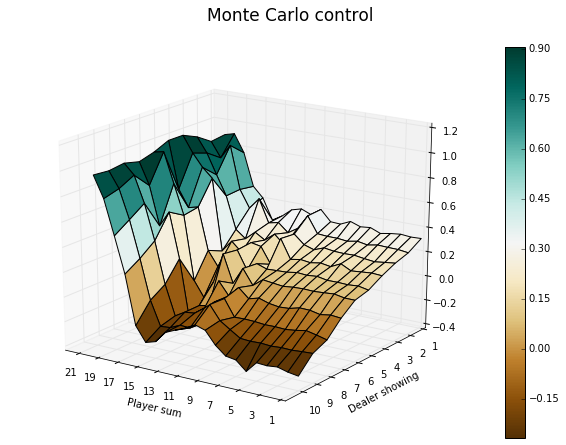
\includegraphics[scale=0.7]{MC}
\end{center}
The Figure show a 3d plot of the dealer's card, player's total and the Q-value for that state.
\\
\\
Result Obtained: Wins, 52.1592\%
\\
\\
Here we have covered Monte Carlo reinforcement learning methods that depending on stochastically sampling the environment and iteratively improving a policy $\pi$ after each episode. One disadvantage of Monte Carlo methods is that we must wait until the end of an episode to update our policy. For some types of problems (like blackjack), this is okay, but in a lot of cases, it makes more sense to able to learn at each time step (immediately after each action is taken).
The whole point of the Monte Carlo simulations were to build an action-value table. The action-value table basically is our  $Q(s,a)$ function. You give it a state and an action and it just goes and looks up the value in the table. The most important thing to learn from all of this is that in essentially any RL method, our goal is to find an optimal Q function. Most of the differences between RL algorithms revolve around differences in determining Q-values. The policy function is straightforward, just pick the best action using $Q(s,a)$.
\\
\\
The next step of the project shows the Mean Square Error $\sum_{s,a}(Q(s, a) −- Q^*(s, a))^2$ over all states $s$ and actions $a$, comparing the values $Q^*(s,a)$ computed in the previous section with the estimated values $Q(s, a)$ computed by Sarsa$(\lambda)$, on 5000 episodes, as we can see in the next Figures.

\begin{center}
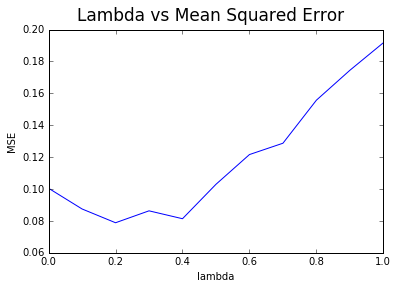
\includegraphics[scale=0.7]{10}
\end{center}

The first figure shows the MSE when $\lambda \in \{0, 0.1, 0.2,\cdots,1\}$, and as we can see, when $\lambda$ assume value 0.4 the MSE become monotonically increasing. In fact, as we cas see in the following figures:

\begin{center}
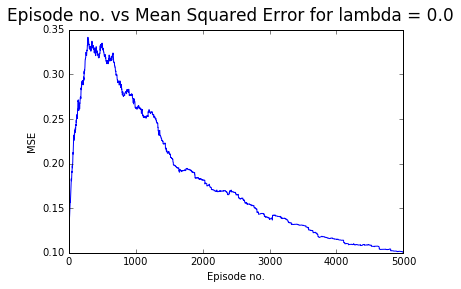
\includegraphics[scale=0.7]{8}
\end{center}
\begin{center}
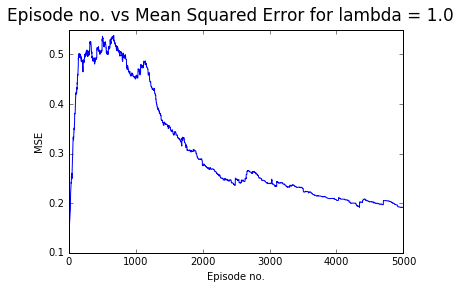
\includegraphics[scale=0.7]{9}
\end{center}

 when $\lambda=1$ the value of MSE is the highest obtained during the execution; it converges at $0.1918$, while when $\lambda$ assumes low values, the MSE converges to a value around $0.0875$.
\\
\\
Successively has been tested the Sarsa$(\lambda)$ Algorithm twenty times and has been evaluated the MSE over all the times. The next Figure shows the result.

\begin{center}
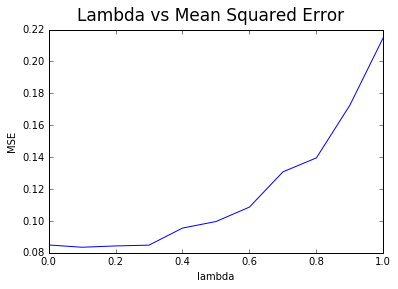
\includegraphics[scale=0.7]{20_mse}
\end{center}

Is important to notice taht the Figure shows that, with the increasing of the value of $\lambda$, the MSE is also increasing.
\section{Conclusions}
Model-free prediction is predicting the value function of a certain policy without a concrete model.

The simplest method is Monte-Carlo learning. However, it only works on episodic tasks: where you have a certain set of actions, the episode ends with some total reward. Monte-Carlo learning states that the return of a state is simply the mean average of the total reward from when a state appeared onwards.

In short, once an episode has concluded, every state that was present can update its value function towards that end return.

However, a problem lies in that every state updates towards the end return, even though that individual state may have had no impact whatsoever on how much reward there was at the end. In order to reduce the variance, we can use a different method of prediction.

Temporal-difference learning, or TD learning, updates the values of each state based on a prediction of the final return. For example, let's say Monte-Carlo learning takes 100 actions and then updates them all based on the final return. TD learning would take an action, and then update the value of the previous action based on the value of the current action. TD learning has the advantage of updating values on more recent trends, in order to capture more of the effect of a certain state.

TD has a lower variance than Monte-Carlo, as each update depends on less factors. However, Monte-Carlo has no bias, as values are updated directly towards the final return, while TD has some bias as values are updated towards a prediction.

TD and Monte-Carlo are actually opposite ends of a spectrum between full lookahead and one-step lookahead. Any number of steps can be taken before passing the return back to an action. One step would be the previously discussed TD learning, and infinite steps is Monte-Carlo as we can see in the next Figure.

\begin{center}
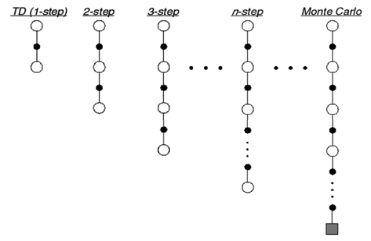
\includegraphics[scale=0.7]{20}
\end{center}

The question rises: how many steps is optimal to look ahead? Unfortunately, it varies greatly depending on the environment and is often a hyperparameter. Another solution is TD(λ), which takes a geometric-weighted average of all n-step lookaheads and uses that to update the value.

Finally, another way to think about TD(λ) is through eligibility traces. An eligibility trace is some weighting that is assigned to every state, based on how frequently and recently it has shown up. After each action, all states are updated proportionally to their eligibility trace towards the reward.

\paragraph{Possible Future Work} could be to consider the aces value equal to eleven and the possibility by player to split his first two cards.
Moreover, could be interesting evaluate this kind of problem with other combination of RL Algorithm's.
\end{document}